\documentclass[11pt,a4paper]{article}

\usepackage[utf8]{inputenc}
\usepackage[T1]{fontenc}
\usepackage{lmodern}
\usepackage[french]{babel}
\usepackage[margin=2.1cm]{geometry}
\usepackage{amsmath,amssymb}
\usepackage{booktabs,tabularx,array,multirow}
\usepackage{graphicx}
\usepackage[table]{xcolor}
\usepackage{tikz}
\usetikzlibrary{arrows.meta,positioning}
\usepackage{tcolorbox}
\tcbuselibrary{skins,breakable}
\usepackage{enumitem}
\usepackage{caption}
\usepackage{float}
\usepackage{fancyhdr}
\usepackage[hidelinks]{hyperref}

\graphicspath{{../reports/figures/}}

\definecolor{bleu}{HTML}{1F4E79}
\definecolor{bleuclair}{HTML}{E8F0F8}
\definecolor{vert}{HTML}{2E7D32}
\definecolor{vertclair}{HTML}{E8F5E9}
\definecolor{orange}{HTML}{E65100}
\definecolor{orangeclair}{HTML}{FFF3E0}
\definecolor{violet}{HTML}{5E35B1}
\definecolor{violetclair}{HTML}{EDE7F6}
\definecolor{gris}{HTML}{F5F5F5}

\newtcolorbox{retenir}[1][À retenir]{colback=bleuclair,colframe=bleu,fonttitle=\bfseries,title={#1},breakable}
\newtcolorbox{analogie}[1][Analogie]{colback=vertclair,colframe=vert,fonttitle=\bfseries,title={#1},breakable}
\newtcolorbox{piege}[1][Piège à éviter]{colback=orangeclair,colframe=orange,fonttitle=\bfseries,title={#1},breakable}
\newtcolorbox{oral}[1][À dire à l'oral]{colback=violetclair,colframe=violet,fonttitle=\bfseries,title={#1},breakable}

\setlist{itemsep=2pt,topsep=4pt}
\renewcommand{\arraystretch}{1.18}
\captionsetup{font=small}

\pagestyle{fancy}
\fancyhf{}
\lhead{\small Guide d'équipe — CAMELYON17}
\rhead{\small \thepage}
\setlength{\headheight}{14pt}

\title{\vspace{-1.3cm}\textbf{\color{bleu}Guide d'équipe : tout comprendre du projet CAMELYON17}\\[4pt]
\large Pour être opérationnel à l'oral, même en partant de zéro en data}
\author{Ali Houaoui \quad Benjamin Gardet \quad Mathys Vrillon \quad Rayan Abdoulkader Houmed}
\date{Document interne, à lire avec le rapport (\texttt{docs/rapport\_final.pdf})}

\begin{document}
\maketitle
\thispagestyle{fancy}

\begin{retenir}[Le projet en 6 phrases]
\begin{enumerate}
  \item On veut aider un médecin à trouver le \textbf{cancer du sein} qui s'est propagé dans les \textbf{ganglions}, sur des images
        au microscope.
  \item \textbf{Étape 1} : un modèle regarde des petits carrés d'image (\emph{patchs}) et dit « cancer » ou « pas cancer ».
  \item On compare un \textbf{CNN} (modèle classique pour les images) à \textbf{Phikon} (gros modèle déjà entraîné sur des millions
        d'images de tissus).
  \item Dans un \textbf{hôpital jamais vu}, le meilleur CNN ne trouve que \textbf{72\,\%} des cancers ; Phikon en trouve \textbf{98\,\%}.
        La raison : les CNN se font piéger par la \textbf{couleur} propre à chaque hôpital.
  \item \textbf{Étape 2} : on applique Phikon à des lames entières pour donner le \textbf{stade pN} de 57 patientes ; la meilleure
        méthode (\textbf{ABMIL hybride}) est d'accord avec les médecins à \textbf{0,89} (kappa, 1 = parfait).
  \item Point faible : les \textbf{toutes petites métastases}. Message éthique : c'est un \textbf{outil d'aide}, pas un remplaçant du médecin.
\end{enumerate}
\end{retenir}

\paragraph{Comment lire ce guide.} Chaque partie explique une notion simplement, avec une analogie, puis donne ce qu'il faut
\textbf{dire à l'oral} (encadrés violets) et les \textbf{pièges} (encadrés orange). La partie~\ref{sec:oral} propose un plan
d'oral de 10 minutes, la partie~\ref{sec:faq} les questions probables de la prof avec les réponses, et la partie~\ref{sec:chiffres}
les chiffres à connaître par cœur.

\begin{table}[H]
\centering\small
\begin{tabularx}{\textwidth}{lX}
\toprule
\textbf{Section du rapport} & \textbf{Où c'est expliqué dans ce guide} \\
\midrule
1. Contexte et objectifs & partie~\ref{sec:medical} \\
2. Données & parties~\ref{sec:vocab} et~\ref{sec:donnees} \\
3. Méthodes & parties~\ref{sec:metriques}, \ref{sec:modeles} et~\ref{sec:etape2} \\
4. Résultats étape 1 (CNN contre Phikon) & partie~\ref{sec:resultats1} \\
5. Résultats étape 2 (stade pN) & partie~\ref{sec:etape2} \\
6. Changement de domaine & partie~\ref{sec:domaine} \\
7. Interprétabilité & partie~\ref{sec:interp} \\
8. Éthique & partie~\ref{sec:ethique} \\
9. Conclusion et limites & partie~\ref{sec:limites} \\
\bottomrule
\end{tabularx}
\end{table}

\tableofcontents
\newpage

%=====================================================================
\section{Le problème médical}\label{sec:medical}
%=====================================================================

\subsection{L'histoire en 5 étapes}
\begin{enumerate}
  \item Une femme a un \textbf{cancer du sein}. Le danger, c'est que le cancer \textbf{voyage} dans le corps.
  \item Sa première étape, ce sont les \textbf{ganglions lymphatiques} de l'aisselle (des petits filtres du système immunitaire).
  \item Le chirurgien retire ces ganglions. Chacun est coupé en tranches très fines, \textbf{coloré} en rose et violet, puis
        photographié au microscope en très haute définition.
  \item On obtient une \textbf{lame entière} : une image géante d'environ $100\,000\times200\,000$ pixels (1 à 3\,Go).
  \item Un médecin spécialiste, le \textbf{pathologiste}, cherche des cellules cancéreuses et \textbf{mesure la taille} de la zone
        atteinte. Une tumeur trouvée dans un ganglion s'appelle une \textbf{métastase}.
\end{enumerate}

\paragraph{La coloration H\&E.} Sans colorant, le tissu est transparent. L'\textbf{hématoxyline} colore les noyaux en
\textbf{violet}, l'\textbf{éosine} colore le reste en \textbf{rose}. Chaque hôpital a sa propre recette et son propre scanner :
\textbf{les couleurs changent d'un hôpital à l'autre}. C'est le fil rouge de tout le projet.

\subsection{La taille de la métastase : 4 classes pour un ganglion}
\begin{table}[H]
\centering
\begin{tabular}{lll}
\toprule
\textbf{Classe du ganglion} & \textbf{Plus grande zone de cancer} & \textbf{En clair} \\
\midrule
Négatif & aucune cellule cancéreuse & sain \\
ITC (cellules tumorales isolées) & moins de 0,2\,mm & quelques cellules perdues \\
Micro-métastase & de 0,2 à 2\,mm & petite métastase \\
Macro-métastase & plus de 2\,mm & métastase installée \\
\bottomrule
\end{tabular}
\end{table}

\subsection{Du ganglion au stade de la patiente : le stade pN}
Une patiente a \textbf{5 ganglions} analysés. Le \textbf{stade pN} résume les 5 ganglions avec des règles officielles :
\begin{table}[H]
\centering
\begin{tabular}{ll}
\toprule
\textbf{Stade} & \textbf{Règle} \\
\midrule
pN0 & aucun ganglion atteint \\
pN0(i+) & seulement des ITC \\
pN1mi & au moins une micro-métastase, aucune macro \\
pN1 & 1 à 3 ganglions atteints, dont au moins une macro \\
pN2 & 4 à 9 ganglions atteints, dont au moins une macro \\
\bottomrule
\end{tabular}
\end{table}

\begin{analogie}[Exemple concret]
Patiente X : ganglion 1 sain, ganglion 2 avec une tache de 1,4\,mm (micro), ganglion 3 sain, ganglion 4 avec 0,1\,mm (ITC),
ganglion 5 sain. Il y a au moins une micro-métastase et aucune macro : \textbf{stade pN1mi}.
\end{analogie}

Le stade décide du traitement (chimiothérapie, radiothérapie\dots). C'est pour ça que c'est important.

\subsection{L'idée qui guide tous nos choix}
\begin{table}[H]
\centering
\begin{tabularx}{\textwidth}{XXl}
\toprule
\textbf{Erreur} & \textbf{Ce qui se passe} & \textbf{Gravité} \\
\midrule
Le modèle dit « cancer » alors que c'est sain & le médecin vérifie pour rien & pas grave \\
Le modèle dit « sain » alors que c'est un cancer & la patiente risque de ne pas être soignée & \textbf{très grave} \\
\bottomrule
\end{tabularx}
\end{table}

\begin{retenir}
On préfère un modèle qui fait quelques \textbf{fausses alertes} plutôt qu'un modèle qui \textbf{rate des cancers}. D'où notre
métrique principale : la \textbf{sensibilité} (part des cancers trouvés).
\end{retenir}

%=====================================================================
\section{Le vocabulaire de base de la data}\label{sec:vocab}
%=====================================================================

\begin{table}[H]
\centering\small
\begin{tabularx}{\textwidth}{lX}
\toprule
\textbf{Mot} & \textbf{Explication simple} \\
\midrule
Donnée / exemple & une image (ici un patch) avec ses informations \\
Étiquette (\emph{label}) & la bonne réponse : 1 = cancer, 0 = sain. C'est le « corrigé » \\
Modèle & un programme qui apprend à donner la bonne réponse à partir d'exemples \\
Paramètres / poids & les nombres internes que le modèle ajuste en apprenant \\
Entraînement & le modèle regarde des exemples avec leur corrigé et corrige ses poids \\
Classification binaire & une question à deux réponses possibles (cancer / pas cancer) \\
Probabilité & le modèle ne répond pas « oui » ou « non », il donne un nombre entre 0 et 1 (« 92\,\% cancer ») \\
Seuil & la valeur à partir de laquelle on dit « cancer » (ex. : si probabilité $\geq$ 0,5) \\
Sur-apprentissage & le modèle apprend ses exemples \textbf{par cœur} au lieu de comprendre ; il échoue sur du nouveau \\
Fuite de données & une information du test « fuit » dans l'entraînement : le score est faussement bon \\
\bottomrule
\end{tabularx}
\end{table}

\subsection{Entraînement, validation, test}
\begin{analogie}[La cuisine]
\textbf{Entraînement} = cuisiner. \textbf{Validation} = goûter soi-même avec une cuillère pour décider (quand arrêter la
cuisson, combien de sel). \textbf{Test} = le jury goûte le plat fini et met une note, \textbf{une seule fois}. On n'a pas le droit
de faire goûter le jury pendant qu'on cuisine, sinon sa note ne veut plus rien dire.
\end{analogie}

\begin{table}[H]
\centering\small
\begin{tabularx}{\textwidth}{lllX}
\toprule
\textbf{Ensemble} & \textbf{Contenu} & \textbf{Rôle} & \textbf{En une phrase} \\
\midrule
\texttt{train} & hôpitaux 0, 3, 4 (80\,\% des patientes) & apprendre & les exercices avec corrigé \\
\texttt{val\_id} & hôpitaux 0, 3, 4 (20\,\% des patientes) & régler & examen blanc dans \emph{son} lycée \\
\texttt{val\_ood} & hôpital 1 & surveiller, choisir le meilleur CNN & examen blanc dans un \emph{autre} lycée \\
\texttt{test\_ood} & hôpital 2 & note finale & le vrai bac, une seule fois \\
\bottomrule
\end{tabularx}
\end{table}
\noindent \textbf{id} = \emph{in distribution} (hôpitaux connus) ; \textbf{ood} = \emph{out of distribution} (hôpital inconnu).

\begin{piege}
La validation (\texttt{val\_id}) contient des hôpitaux \textbf{déjà vus} mais des \textbf{patientes jamais vues}. Ce n'est pas la
même chose que le train.
\end{piege}

%=====================================================================
\section{Les données}\label{sec:donnees}
%=====================================================================

\subsection{Ce qu'on a}
\begin{itemize}
  \item \textbf{Camelyon17-WILDS} : \textbf{455\,954 patchs} (petits carrés) de $96\times96$ pixels, environ 0,1\,mm de tissu chacun.
  \item Ils viennent de \textbf{50 lames} (une lame = un ganglion), \textbf{43 patientes}, \textbf{5 hôpitaux} néerlandais.
  \item \textbf{10 lames par hôpital} : ce sont celles où les médecins ont \textbf{dessiné à la main le contour des tumeurs}.
  \item Chaque patch a une étiquette : 1 si son centre est dans une zone dessinée, 0 sinon.
  \item Les chercheurs de WILDS ont \textbf{déjà découpé} les lames pour nous. On télécharge les patchs prêts à l'emploi depuis une copie
        sur Hugging Face (le serveur officiel avait un certificat expiré).
\end{itemize}

\paragraph{Une ligne = un patch.} Chaque patch, c'est une image + une fiche : patiente, ganglion, hôpital, position dans la lame,
étiquette. Les données sont \textbf{anonymes}.

\paragraph{Une image = des nombres.} Une image $96\times96$ en couleur, c'est $96\times96\times3$ nombres de 0 à 255 : chaque pixel a
3 valeurs (rouge, vert, bleu).

\begin{piege}
\textbf{Patch} = une petite image. \textbf{Batch} (lot) = un paquet de patchs (256) donnés ensemble au modèle pendant
l'entraînement. Les deux mots se ressemblent mais n'ont rien à voir.
\end{piege}

\subsection{Pourquoi ce jeu de données}
\begin{enumerate}
  \item Un \textbf{vrai problème médical}, avec des réponses fiables dessinées par des experts.
  \item \textbf{5 hôpitaux} aux couleurs différentes : on peut tester si un modèle marche dans un hôpital qu'il ne connaît pas.
  \item Déjà découpé en patchs et de taille raisonnable (10,7\,Go) : utilisable sur Google Colab gratuit.
  \item Des résultats publiés pour se comparer.
\end{enumerate}
Les lames originales (plusieurs téraoctets) étaient trop lourdes ; PatchCamelyon, une autre version, n'a que 2 hôpitaux.

\subsection{Ce que l'exploration nous a appris}
\begin{enumerate}
  \item \textbf{Données propres} : même format partout, aucune valeur manquante.
  \item \textbf{50\,\% cancer / 50\,\% sain} : c'est artificiel (choix de WILDS). Sur une vraie lame, le cancer fait souvent moins de 1\,\%.
  \item \textbf{La couleur trahit l'hôpital} : avec seulement 6 mesures de couleur, un modèle simple reconnaît l'hôpital dans
        \textbf{80\,\%} des cas (le hasard donnerait 20\,\%). L'hôpital 2 est nettement plus violet.
  \item \textbf{Les patchs cancer sont collés les uns aux autres} sur la lame : deux voisins sont presque identiques.
\end{enumerate}

\begin{figure}[H]
\centering
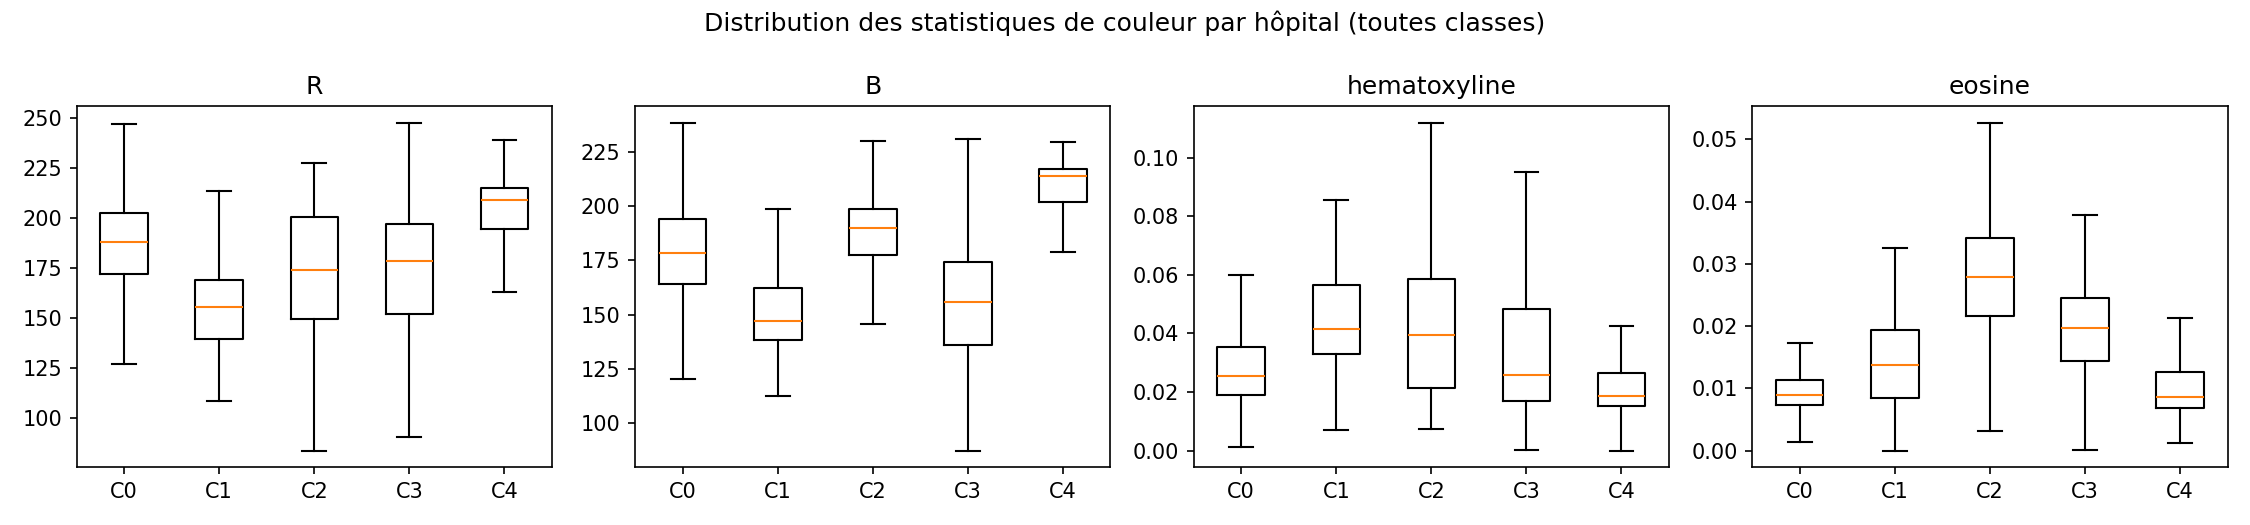
\includegraphics[width=0.49\textwidth]{couleur_par_centre.png}\hfill
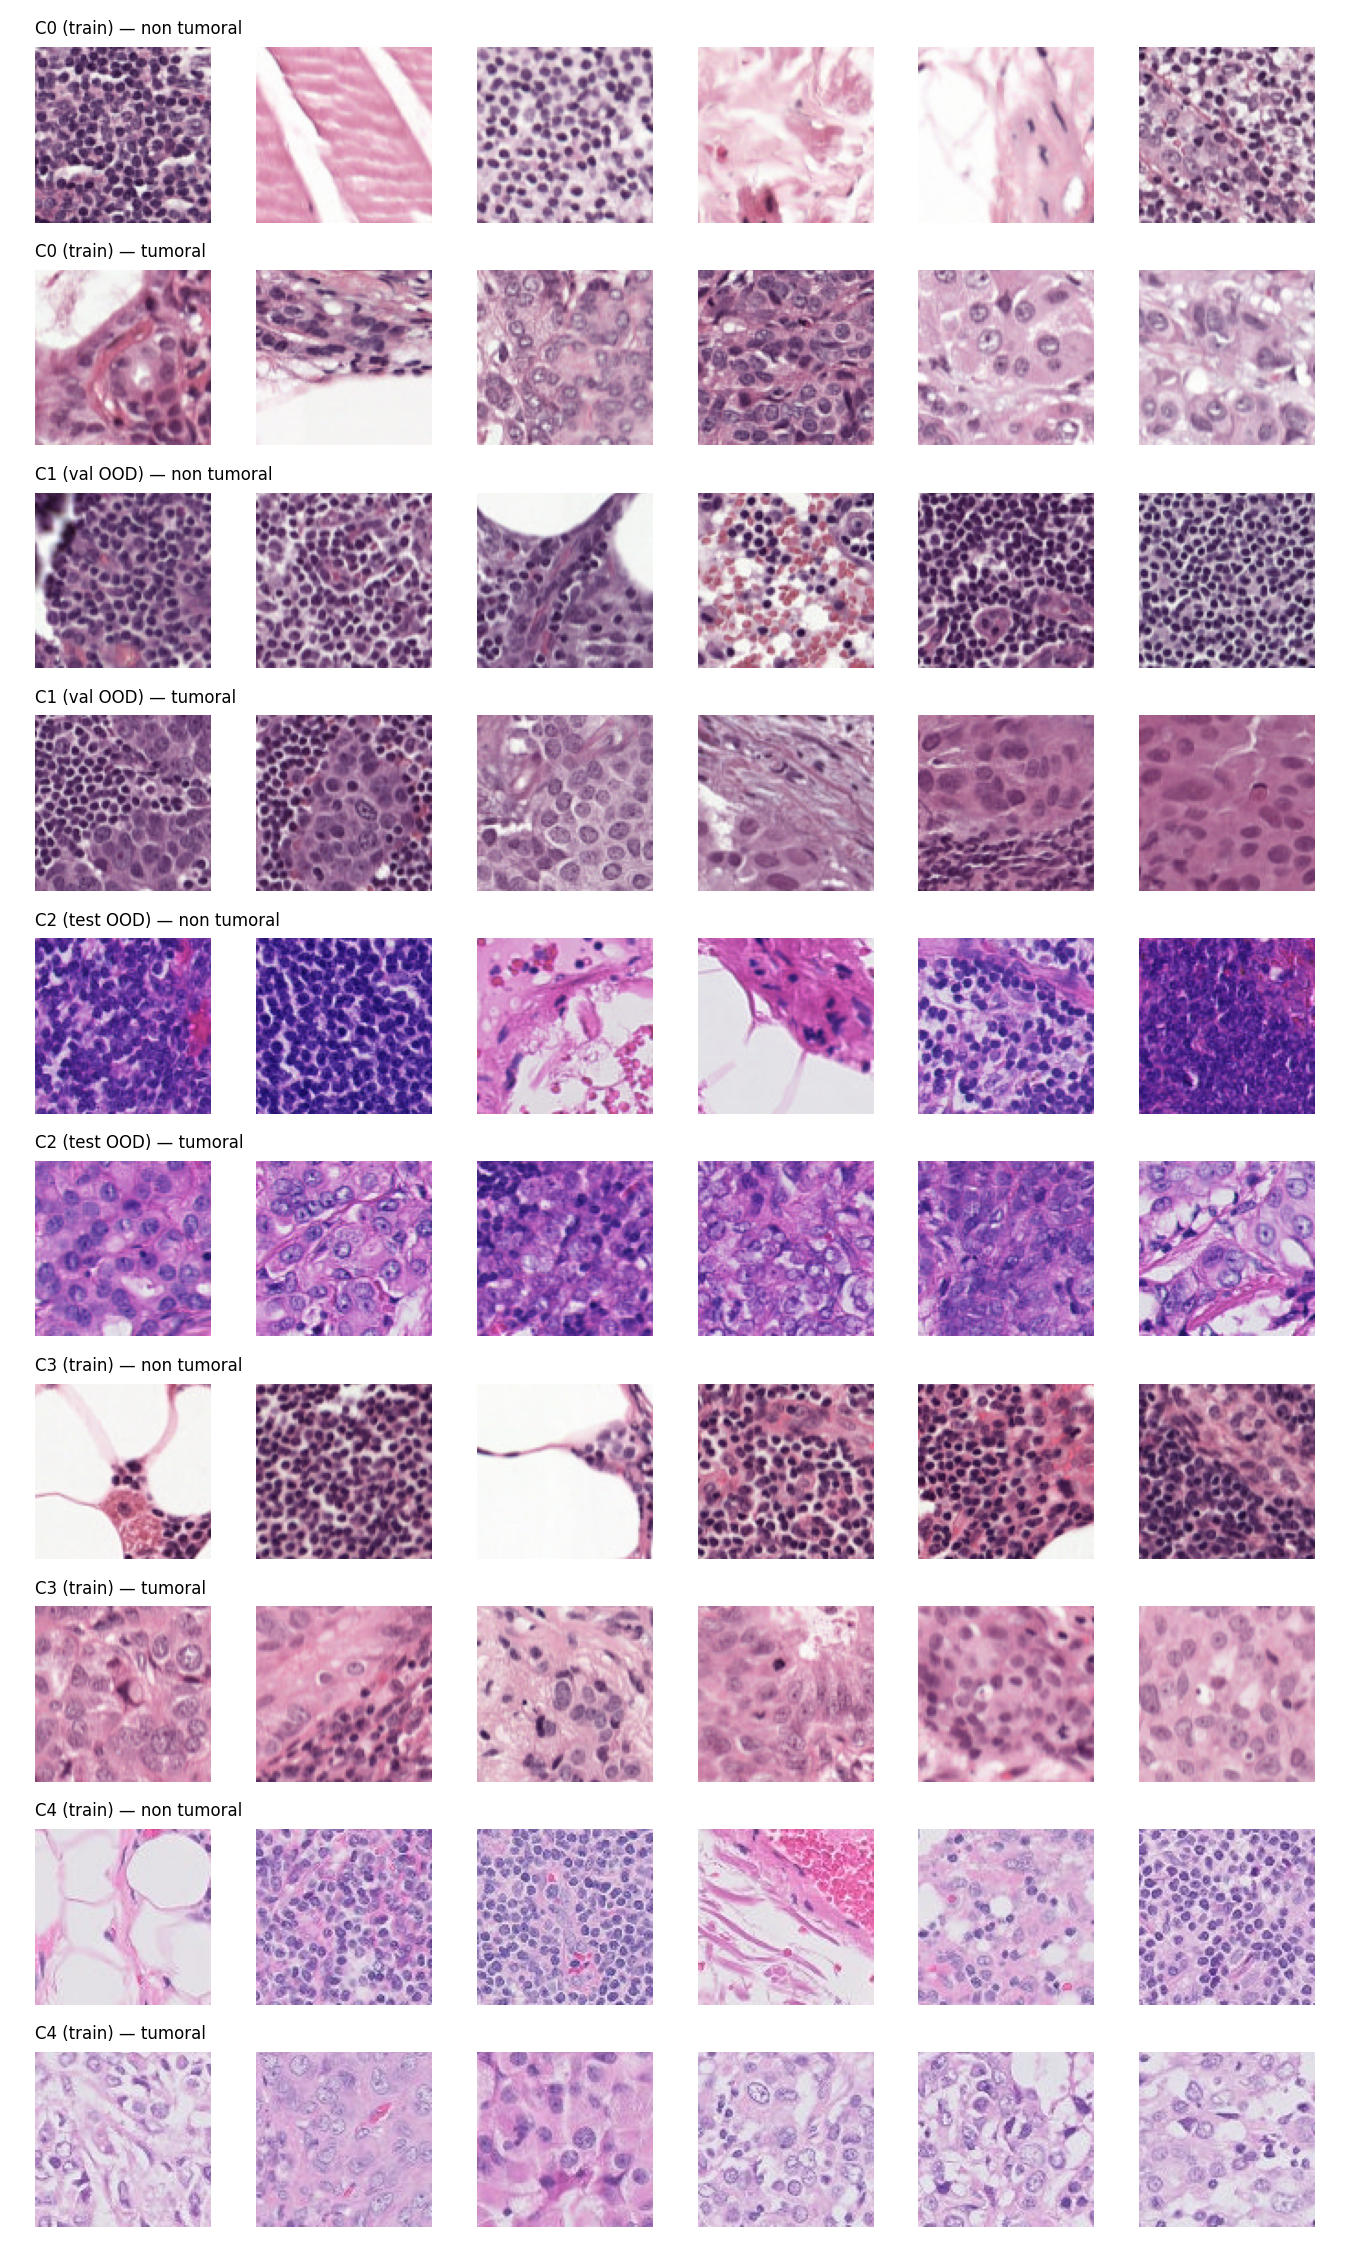
\includegraphics[width=0.49\textwidth]{galerie.png}
\caption{À gauche : la couleur selon l'hôpital. À droite : des patchs sains et cancéreux de chaque hôpital.}
\end{figure}

\subsection{Le découpage sans triche}
\begin{itemize}
  \item \textbf{Par patiente} : toutes les images d'une patiente vont du même côté. Sinon, deux patchs voisins presque identiques
        pourraient être l'un à l'entraînement, l'autre au test : le modèle « reconnaîtrait » l'image au lieu de la comprendre
        (\textbf{fuite de données}). Un contrôle automatique dans le code vérifie qu'aucune patiente n'est dans deux ensembles.
  \item \textbf{Par hôpital} : entraînement sur les hôpitaux 0, 3, 4 ; test sur les hôpitaux 1 et 2, \textbf{jamais vus}. C'est le
        découpage officiel de WILDS, et c'est la situation réelle d'un nouvel hôpital qui achèterait le modèle.
\end{itemize}

\begin{oral}
« On a découpé \textbf{par patiente} pour éviter la fuite de données, et \textbf{par hôpital} pour tester le modèle sur des hôpitaux
qu'il n'a jamais vus, ce qui simule un vrai déploiement. »
\end{oral}

%=====================================================================
\section{Les métriques : comment on note un modèle}\label{sec:metriques}
%=====================================================================

\subsection{La matrice de confusion}
\begin{table}[H]
\centering
\small\begin{tabular}{lcc}
\toprule
 & \textbf{le modèle dit SAIN} & \textbf{le modèle dit CANCER} \\
\midrule
\textbf{c'est vraiment SAIN} & VN (vrai négatif) & FP (faux positif = fausse alerte) \\
\textbf{c'est vraiment CANCER} & \cellcolor{orangeclair}FN (faux négatif = \textbf{cancer raté}) & VP (vrai positif) \\
\bottomrule
\end{tabular}
\end{table}

\subsection{Les métriques}
\begin{table}[H]
\centering\small
\begin{tabularx}{\textwidth}{llX}
\toprule
\textbf{Métrique} & \textbf{Formule} & \textbf{Question à laquelle elle répond} \\
\midrule
\textbf{Sensibilité} & VP / (VP + FN) & parmi les vrais cancers, combien sont trouvés ? \textbf{Notre priorité.} \\
Spécificité & VN / (VN + FP) & parmi les tissus sains, combien sont bien reconnus ? (mesure les fausses alertes) \\
Exactitude & (VP + VN) / total & combien de bonnes réponses ? \textbf{Trompeuse} si le cancer est rare \\
AUC & aire sous la courbe ROC & les cancers sont-ils \textbf{rangés au-dessus} des sains ? (0,5 = hasard, 1 = parfait) \\
\bottomrule
\end{tabularx}
\end{table}

\subsection{L'AUC : le point qui piège tout le monde}
\begin{piege}[L'AUC n'est pas un pourcentage de bonnes réponses]
L'AUC dit si le modèle \textbf{range} bien les patchs : est-ce que les cancers ont une probabilité plus haute que les sains ?
Elle ne dit \textbf{pas} combien de décisions sont justes, car elle ne dépend pas du seuil.
\end{piege}

\begin{analogie}[Le thermomètre décalé]
Un thermomètre affiche toujours 2\,°C de moins que la réalité. Il \textbf{range} parfaitement les patients du plus chaud au moins
chaud (AUC parfaite). Mais avec la règle « fièvre si $\geq$ 38\,°C », il rate des fièvres (mauvaise décision). C'est exactement
ce qui arrive au CNN sur l'hôpital 2 : bonne AUC, mais beaucoup de cancers ratés.
\end{analogie}

\subsection{Le seuil réglé à 95\,\% de sensibilité}
Le modèle donne une probabilité. On règle le \textbf{seuil} sur les hôpitaux d'entraînement pour trouver \textbf{95\,\% des cancers},
puis on l'applique \textbf{tel quel} aux hôpitaux 1 et 2. C'est réaliste : dans un nouvel hôpital, on ne peut pas régler le seuil sur
les patientes qu'on est en train de diagnostiquer.

\subsection{L'intervalle de confiance (IC)}
Un chiffre seul peut être dû au hasard (quelles patientes sont dans le test). On refait le calcul 1\,000 fois en tirant des patientes au
hasard (\textbf{bootstrap}) et on donne la fourchette qui contient 95\,\% des résultats. \textbf{Un IC large = résultat peu sûr.}
On tire des \textbf{patientes} et non des patchs, car les patchs d'une même patiente se ressemblent trop.

\subsection{Le kappa (pour le stade, étape 2)}
Le \textbf{kappa pondéré quadratique} mesure l'\textbf{accord} entre notre stade et celui des médecins : 1 = accord parfait, 0 = comme
le hasard. « Pondéré » : une erreur de 2 crans (pN0 au lieu de pN1) coûte 4 fois plus qu'une erreur d'un cran. Au-delà de 0,8, on
parle d'accord « presque parfait ». C'est la métrique officielle du challenge.

%=====================================================================
\section{Les modèles de l'étape 1}\label{sec:modeles}
%=====================================================================

\subsection{Comment un modèle apprend (pour tous les réseaux)}
\begin{enumerate}
  \item On lui montre un \textbf{lot} de 256 images.
  \item Il donne ses réponses (probabilités).
  \item La \textbf{fonction de perte} (entropie croisée) \textbf{mesure} son erreur : elle punit fort les erreurs commises avec assurance.
  \item La \textbf{rétropropagation} \textbf{calcule} dans quel sens corriger chacun de ses poids.
  \item L'\textbf{optimiseur} (AdamW) \textbf{corrige} les poids d'un petit pas.
  \item On recommence. Une \textbf{époque} = toutes les images d'entraînement vues une fois.
\end{enumerate}
\begin{analogie}[Les fléchettes]
On lance (prédiction), on regarde à quelle distance du centre on est (perte), on comprend comment ajuster son geste
(rétropropagation), on ajuste (optimiseur), et on recommence des milliers de fois.
\end{analogie}

\subsection{Le CNN (réseau de neurones convolutif)}
\begin{itemize}
  \item Un CNN fait glisser de petits \textbf{filtres} ($3\times3$ pixels) sur l'image. Chaque filtre détecte un motif : un bord,
        une texture, puis, en empilant les couches, des formes complexes (un noyau, un amas de cellules).
  \item Les nombres dans les filtres sont \textbf{appris} pendant l'entraînement.
  \item Briques : convolution (filtres), normalisation (stabilise), ReLU (permet d'apprendre des formes complexes), pooling (réduit la
        taille), dropout (éteint des neurones au hasard contre le par-cœur), couche finale (2 scores, transformés en probabilités par
        le softmax).
\end{itemize}

\paragraph{Nos 4 CNN.}
\begin{table}[H]
\centering\small
\begin{tabularx}{\textwidth}{lX}
\toprule
\textbf{CNN} & \textbf{Ce que c'est} \\
\midrule
Petit CNN & 4 blocs de convolution, 389\,000 paramètres, appris \textbf{de zéro} (c'est celui du notebook Colab) \\
ResNet18 & un CNN de 18 couches, 11 millions de paramètres, \textbf{pré-entraîné} sur ImageNet (1,2 million de photos ordinaires :
chats, voitures\dots), puis ré-entraîné sur nos patchs (\emph{fine-tuning}). Ses « raccourcis » (connexions résiduelles) permettent
d'empiler beaucoup de couches \\
Petit CNN + HED & le petit CNN avec une \textbf{augmentation de couleur} à l'entraînement \\
ResNet18 + HED & le ResNet18 avec l'augmentation de couleur \\
\bottomrule
\end{tabularx}
\end{table}

\paragraph{L'augmentation HED.} À chaque lot, on modifie un peu au hasard la quantité de violet (hématoxyline) et de rose (éosine)
de chaque image. Le modèle voit des couleurs variées et doit apprendre la \textbf{forme} des cellules plutôt que leur couleur. On y
ajoute des rotations et des miroirs (un tissu n'a ni haut ni bas).

\paragraph{Le meilleur CNN.} On l'a choisi sur l'\textbf{hôpital 1} (jamais sur l'hôpital 2, qui est le test) : c'est le
\textbf{ResNet18 + HED} (meilleure AUC sur l'hôpital 1 : 0,985).

\subsection{Phikon (le modèle de fondation)}
\begin{itemize}
  \item \textbf{Ce n'est pas un CNN}, ni un LLM (texte), ni un VLM (image + texte). C'est un \textbf{modèle de vision} de type
        \textbf{Vision Transformer} (ViT), créé par Owkin (entreprise française), 86 millions de paramètres.
  \item Il a été \textbf{pré-entraîné} sur des millions d'images de tissus de nombreux cancers et hôpitaux, \textbf{sans étiquette}
        (\textbf{auto-supervision} : on cache des morceaux d'image et il apprend à deviner ce qui manque).
  \item On l'utilise \textbf{figé} : on ne touche pas à ses poids. Il transforme chaque patch en une \textbf{fiche de 768 nombres}
        qui décrit le tissu (noyaux, organisation, texture).
  \item Par-dessus, une \textbf{régression logistique} (la « sonde », 769 paramètres) lit la fiche et donne la probabilité de cancer.
\end{itemize}

\begin{analogie}[Le pathologiste et le médecin qui décide]
Phikon est un pathologiste très expérimenté qui \textbf{décrit} chaque image (une fiche de 768 cases), sans dire si c'est un cancer.
La régression logistique est le médecin qui \textbf{lit la fiche} et tranche. On n'entraîne que ce deuxième médecin, en quelques minutes.
\end{analogie}

\begin{table}[H]
\centering\small
\begin{tabularx}{\textwidth}{lXX}
\toprule
 & \textbf{CNN} & \textbf{Phikon + régression logistique} \\
\midrule
Comment il regarde & des filtres $3\times3$ qui glissent & découpe l'image en morceaux reliés par « attention » \\
Ce qu'on entraîne & tout le réseau (389\,k à 11\,M poids) & seulement la régression logistique (769 poids) \\
Ce qu'il a vu avant & rien, ou des photos ordinaires & des millions d'images de tissus de nombreux hôpitaux \\
\bottomrule
\end{tabularx}
\end{table}

\begin{piege}
Le nom est \textbf{Phikon}, pas « Phi-3 » (Phi-3 est un modèle de texte de Microsoft, sans rapport).
\end{piege}

\subsection{Les autres modèles (complémentaires)}
Pour situer nos deux approches, on a aussi testé : deux modèles \textbf{classiques} (statistiques de couleur et de texture, puis
régression logistique ou forêt aléatoire), et trois autres modèles de fondation (\textbf{Phikon-v2}, \textbf{Midnight},
\textbf{DINOv2}). Ils ne sont pas au cœur de l'oral, mais il faut savoir qu'ils existent.

%=====================================================================
\section{Les résultats de l'étape 1 : CNN contre Phikon}\label{sec:resultats1}
%=====================================================================

\begin{table}[H]
\centering\small
\begin{tabular}{lccc}
\toprule
 & \multicolumn{2}{c}{\textbf{Cancers trouvés}} & \textbf{Patchs cancer} \\
\textbf{Modèle} & \textbf{hôpital 1} & \textbf{hôpital 2} & \textbf{ratés (hôpital 2)} \\
\midrule
Meilleur CNN (ResNet18 + HED) & 88\,\% & \textbf{72\,\%} & 11\,881 \\
\rowcolor{bleuclair}\textbf{Phikon + régression logistique} & \textbf{98\,\%} & \textbf{98\,\%} & \textbf{705} \\
\bottomrule
\end{tabular}
\end{table}

\begin{figure}[H]
\centering
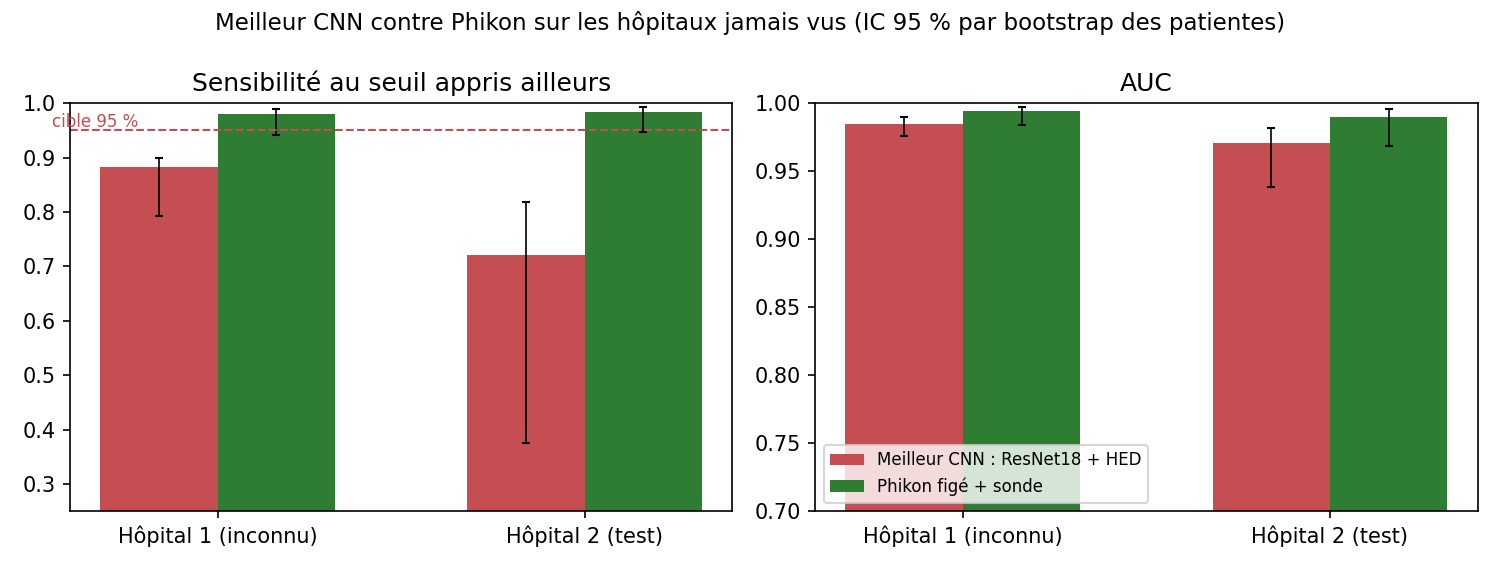
\includegraphics[width=0.9\textwidth]{cnn_vs_phikon.png}
\caption{Le graphique du rapport : à gauche les cancers trouvés, à droite l'AUC.}
\end{figure}

\paragraph{Comment lire ce résultat.}
\begin{enumerate}
  \item Sur ses propres hôpitaux, le CNN est excellent (AUC $\geq$ 0,99). Le problème n'apparaît que dans un \textbf{nouvel hôpital}.
  \item Le CNN \textbf{range} encore bien les patchs de l'hôpital 2 (AUC 0,971), mais ses probabilités sont décalées par la couleur :
        le seuil réglé chez nous ne convient plus, il rate 28\,\% des cancers.
  \item Phikon reste fiable sur \textbf{les deux} hôpitaux inconnus. Son seul défaut : un peu plus de fausses alertes (spécificité 0,83).
        Pour un outil de tri, c'est le bon compromis.
  \item Il est aussi beaucoup moins coûteux à entraîner (769 paramètres contre 11 millions).
\end{enumerate}

\paragraph{Pourquoi Phikon gagne (3 raisons).}
\begin{enumerate}
  \item Il a déjà vu des tissus de \textbf{très nombreux hôpitaux}, donc beaucoup de colorations différentes.
  \item On n'apprend \textbf{presque rien} sur nos 3 hôpitaux (juste la régression logistique), donc il ne peut pas s'y spécialiser.
  \item Il est pré-entraîné \textbf{en pathologie} : DINOv2, pré-entraîné sur des photos, fait plus de fausses alertes.
\end{enumerate}

\begin{oral}
« Notre CNN est excellent sur ses hôpitaux, mais dans un hôpital jamais vu il ne trouve plus que \textbf{72\,\%} des cancers, car il
se fait piéger par la couleur. \textbf{Phikon}, un modèle de fondation pré-entraîné sur des millions d'images de tissus, en trouve
\textbf{98\,\%} sur les deux hôpitaux inconnus. »
\end{oral}

\begin{piege}[Si la prof demande « pourquoi ce CNN-là ? »]
« Parce qu'on a choisi le meilleur CNN sur l'\textbf{hôpital 1} (validation), jamais sur l'hôpital 2 (test). Le petit CNN + HED fait
95\,\% sur l'hôpital 2, mais seulement 89\,\% sur l'hôpital 1, et le choisir au vu du test serait de la triche. »
\end{piege}

%=====================================================================
\section{L'étape 2 : du patch au stade de la patiente}\label{sec:etape2}
%=====================================================================

\subsection{La chaîne complète, pas à pas}
\begin{figure}[H]
\centering
\begin{tikzpicture}[node distance=0.42cm and 0.4cm, every node/.style={font=\small},
  box/.style={draw=bleu, fill=bleuclair, rounded corners, align=center, minimum height=1cm, text width=2.35cm},
  arr/.style={-{Stealth[length=2.3mm]}, thick, bleu}]
\node[box] (wsi) {Lame entière\\(1 ganglion)};
\node[box, right=of wsi] (tiles) {Découpe en\\tuiles $96{\times}96$};
\node[box, right=of tiles] (phikon) {Phikon :\\768 nombres};
\node[box, right=of phikon] (map) {Rég. logistique :\\carte de chaleur};
\node[box, below=0.9cm of map, fill=vertclair, draw=vert] (cls) {Classe du\\ganglion};
\node[box, left=of cls, fill=vertclair, draw=vert] (pn) {Règles pN\\(5 ganglions)};
\node[box, left=of pn, fill=orangeclair, draw=orange] (stage) {Stade pN\\de la patiente};
\draw[arr] (wsi) -- (tiles); \draw[arr] (tiles) -- (phikon); \draw[arr] (phikon) -- (map);
\draw[arr] (map) -- node[right, align=left, font=\scriptsize]{4 techniques\\comparées} (cls);
\draw[arr] (cls) -- (pn); \draw[arr] (pn) -- (stage);
\end{tikzpicture}
\end{figure}

\begin{enumerate}
  \item \textbf{Les données} : 57 nouvelles patientes (aucune n'a servi à l'étape 1), 5 ganglions chacune, soit 285 lames. Les lames
        (2\,Go) ne sont pas téléchargées : on lit à distance seulement les morceaux qui contiennent du tissu.
  \item \textbf{Découpe} : on repère le tissu (on ignore le fond blanc) et on le découpe en \textbf{tuiles} de $96\times96$, comme les
        patchs. Une lame donne des milliers de tuiles (3 millions au total).
  \item \textbf{Phikon} décrit chaque tuile (768 nombres), la \textbf{régression logistique} donne sa probabilité de cancer.
  \item \textbf{Carte de chaleur} : on remet chaque tuile à sa place sur la lame et on la colorie selon sa probabilité. On voit
        \textbf{où} est le cancer et \textbf{quelle taille} il fait.
  \item \textbf{Classe du ganglion} (sain, ITC, micro, macro) : c'est ici qu'on compare \textbf{4 techniques} (ci-dessous).
  \item \textbf{Stade} : les règles officielles sur les 5 ganglions (aucun modèle à cette étape).
\end{enumerate}

\begin{figure}[H]
\centering
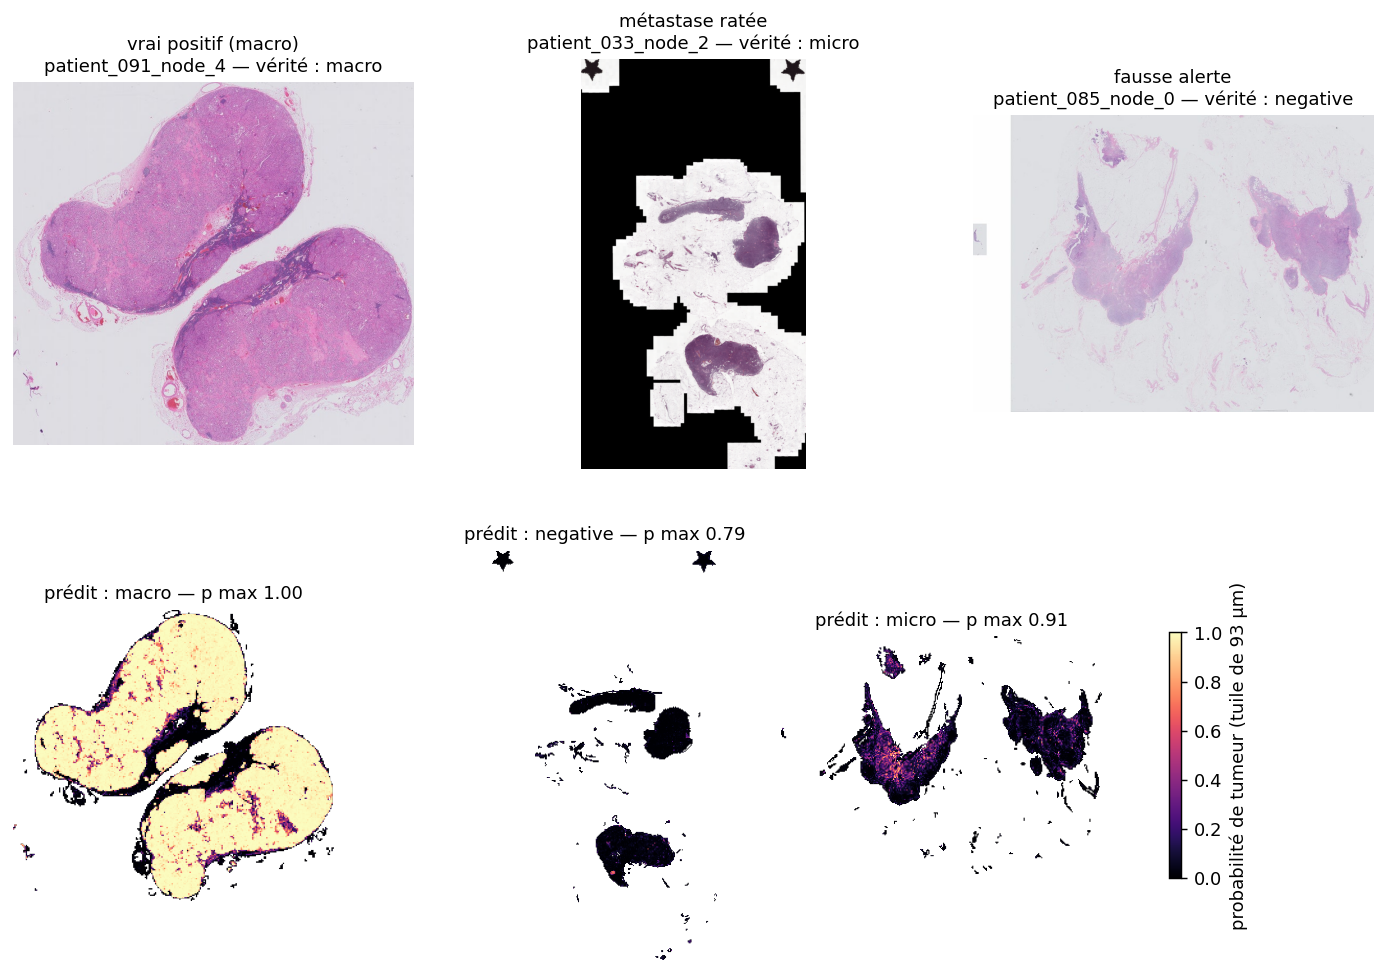
\includegraphics[width=0.9\textwidth]{pn_cartes_exemples.png}
\caption{Des cartes de chaleur : un cancer bien trouvé, une métastase ratée, une fausse alerte.}
\end{figure}

\subsection{Les 4 techniques pour classer un ganglion}
\begin{table}[H]
\centering\small
\begin{tabularx}{\textwidth}{lXc}
\toprule
\textbf{Technique} & \textbf{Comment elle lit la carte de chaleur} & \textbf{Kappa} \\
\midrule
Règle de taille & on garde les tuiles très suspectes, on mesure le plus grand diamètre de la tache en mm, puis les seuils
médicaux 0,2 et 2\,mm. Entièrement explicable & 0,80 \\
Forêt aléatoire & 300 arbres de décision qui votent, à partir de résumés de la carte (probabilité max, nombre de tuiles
suspectes, taille\dots). C'est la méthode des gagnants du challenge & 0,80 \\
ABMIL 3 classes & réseau qui regarde toutes les tuiles et apprend lui-même lesquelles sont importantes (attention) ; il prédit
directement sain / micro / macro & 0,87 \\
\rowcolor{bleuclair}\textbf{ABMIL hybride} & l'ABMIL décide seulement « ganglion atteint ou non » ; la \textbf{taille} vient de la
règle de taille & \textbf{0,89} \\
\bottomrule
\end{tabularx}
\end{table}

\paragraph{L'ABMIL, simplement.} Une lame = un « sac » de milliers de tuiles, mais on n'a qu'une seule réponse pour toute la lame.
L'ABMIL donne un \textbf{poids d'attention} à chaque tuile (« à quel point cette tuile compte pour décider ? »), fait une moyenne
pondérée, puis décide.
\begin{analogie}[Le pathologiste qui survole la lame]
Il ne regarde pas les 30\,000 tuiles avec la même attention : il repère les zones suspectes et se concentre dessus. C'est
l'attention. Et elle s'apprend toute seule.
\end{analogie}

\paragraph{Pourquoi « hybride » ?} L'attention fait une \textbf{moyenne} : elle ne sait pas \textbf{mesurer une taille}. Or, pour
distinguer micro (0,2–2\,mm) et macro ($>$ 2\,mm), il faut mesurer. On combine donc : l'ABMIL pour « atteint ou non » (ce qu'il fait
bien), la règle de taille pour « quelle taille ».

\subsection{Les résultats}
\begin{itemize}
  \item L'\textbf{ABMIL hybride} est le meilleur : kappa \textbf{0,89}, contre 0,80 pour la règle et la forêt, et il gagne \textbf{dans
        les 10 répétitions sur 10} (écart +0,08, IC [0,01 ; 0,18] : l'écart est solide).
  \item Il rate moins de patientes métastatiques (4,4 sur 57 contre 6,4) et fait 3 fois moins de fausses alertes.
  \item Les cancers avancés sont bien classés ; \textbf{le point faible, ce sont les micro-métastases et les ITC} (plus petites qu'une tuile).
  \item Évaluation : validation croisée par patiente (3 groupes, on entraîne sur 2 et on teste sur le 3\textsuperscript{e}, en tournant),
        répétée 10 fois avec des découpages différents.
\end{itemize}

\begin{oral}
« Pour l'étape 2, Phikon nous donne une carte de chaleur de chaque ganglion. On a comparé quatre techniques pour classer le ganglion,
puis les règles officielles donnent le stade. La meilleure est l'\textbf{ABMIL hybride}, avec un kappa de \textbf{0,89}. »
\end{oral}

%=====================================================================
\section{Le changement de domaine}\label{sec:domaine}
%=====================================================================

\paragraph{Définition.} Le \textbf{domaine}, c'est l'hôpital (sa couleur, son scanner). Le \textbf{changement de domaine}, c'est quand
les données d'utilisation ne ressemblent pas aux données d'entraînement, et que le modèle marche moins bien.

\paragraph{Pourquoi la couleur gêne le CNN.} Un ordinateur ne « voit » pas des formes, il lit des \textbf{nombres de couleur}. La même
cellule cancéreuse, colorée plus violet à l'hôpital 2, donne \textbf{d'autres nombres}. Le CNN, qui a appris avec les couleurs de ses
3 hôpitaux, est perdu.
\begin{analogie}[Le filtre Instagram]
On apprend à reconnaître un ami sur des photos normales ; on le montre ensuite avec un filtre violet très fort. Un humain le
reconnaît ; un modèle mal entraîné peut ne pas le reconnaître. Les hôpitaux sont des filtres, le cancer est l'ami.
\end{analogie}

\paragraph{Ce qu'on a mesuré.} La couleur reconnaît l'hôpital à 80\,\% (la cause) ; l'AUC baisse dans les hôpitaux inconnus ; surtout,
la sensibilité au seuil transféré s'effondre (72\,\% pour le meilleur CNN). Et \textbf{plus on entraîne longtemps, plus le CNN se
spécialise} sur ses hôpitaux (dans le notebook à 300 époques : 35\,\% seulement sur l'hôpital 2).

\paragraph{Les deux remèdes testés.}
\begin{enumerate}
  \item \textbf{Changer de modèle : Phikon} $\to$ le plus efficace (98\,\% partout).
  \item \textbf{Augmentation de couleur HED} $\to$ aide beaucoup le petit CNN (82\,\% $\to$ 95\,\% sur l'hôpital 2), très peu le
        ResNet18 (69\,\% $\to$ 72\,\%). Résultat \textbf{exploratoire} (une seule graine).
\end{enumerate}

\begin{piege}
Tester sur des hôpitaux jamais vus ne \textbf{corrige} pas le problème : ça permet de le \textbf{mesurer}. Les remèdes, ce sont
Phikon et l'augmentation de couleur.
\end{piege}

%=====================================================================
\section{L'interprétabilité}\label{sec:interp}
%=====================================================================
\paragraph{Grad-CAM.} Une méthode qui colore les zones de l'image qui ont poussé le modèle à dire « cancer » (rouge = important).
On l'a appliquée au ResNet18 sur l'hôpital 2.
\begin{itemize}
  \item Sur les cancers bien trouvés, il regarde les amas de grosses cellules : la bonne chose.
  \item Sans augmentation de couleur, les cancers ratés sont des patchs \textbf{très sombres et violets} : le modèle n'y voit rien.
        C'est la couleur qui le piège.
  \item Avec l'augmentation de couleur, les cancers ratés sont plutôt \textbf{quelques cellules isolées dans de la graisse} : l'erreur
        devient « normale » (peu de cellules), plus liée à la couleur.
\end{itemize}
\begin{figure}[H]
\centering
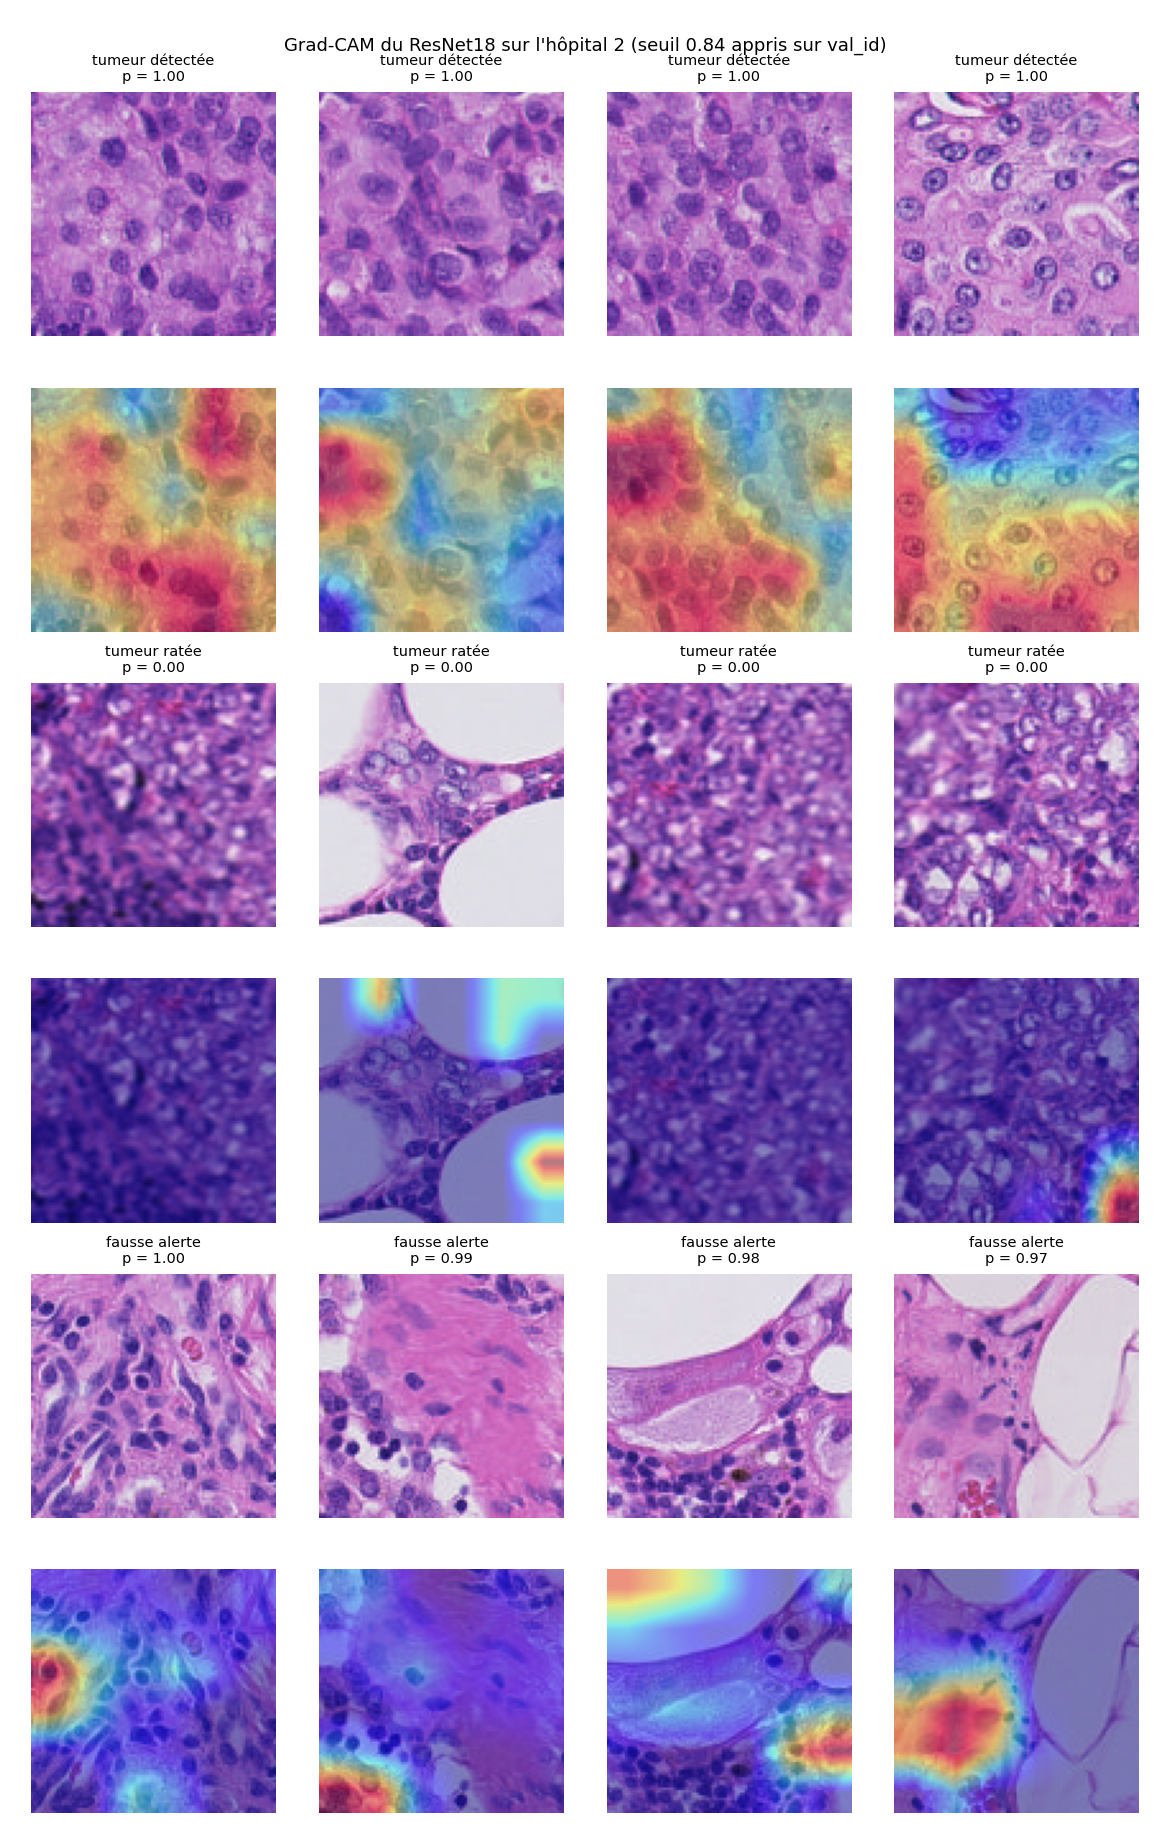
\includegraphics[width=0.42\textwidth]{gradcam_c2_ref.png}\hspace{0.5cm}
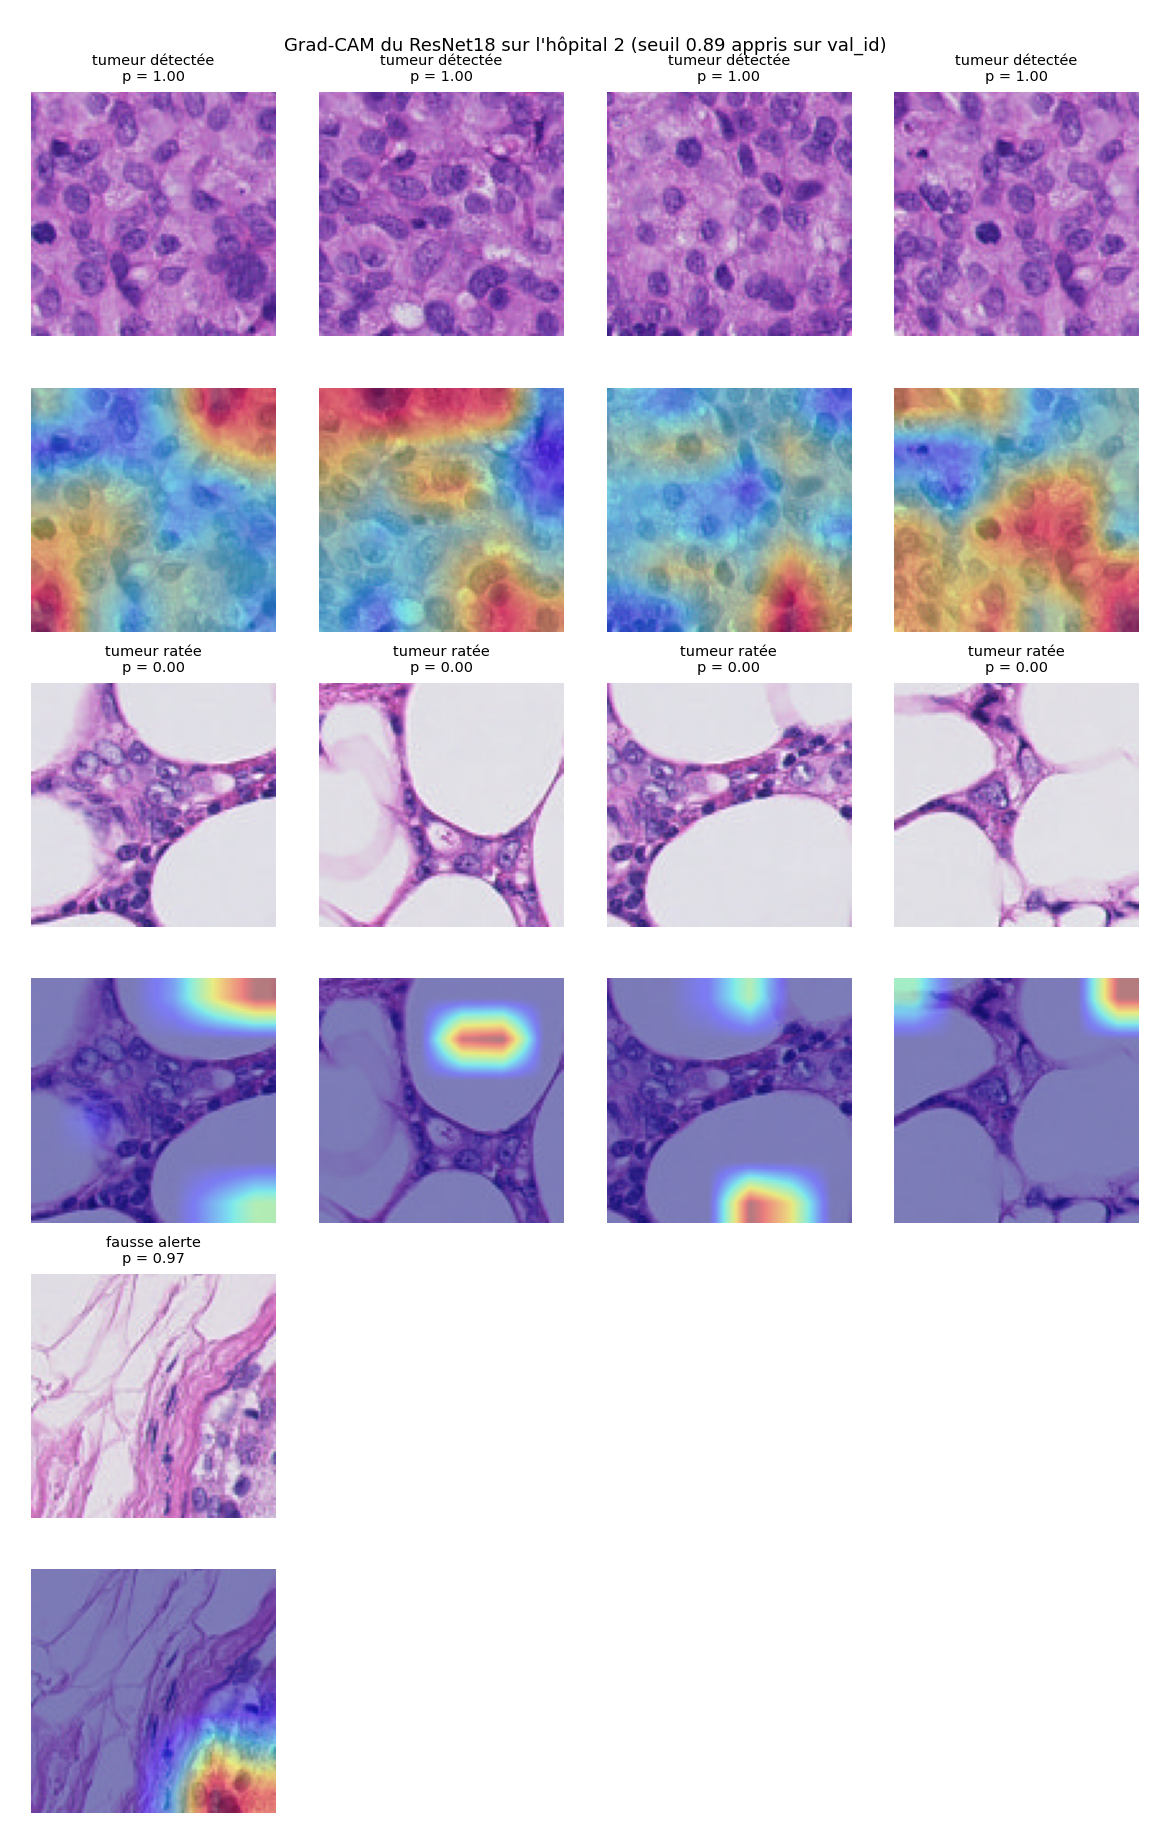
\includegraphics[width=0.42\textwidth]{gradcam_c2_hed.png}
\caption{Grad-CAM sans (à gauche) et avec augmentation de couleur (à droite).}
\end{figure}
\paragraph{Pour l'étape 2,} les \textbf{cartes de chaleur} montrent au médecin où le modèle voit le cancer, et la règle de taille
est explicable par construction.
\begin{piege}
Grad-CAM et l'attention montrent \textbf{où} le modèle regarde, pas \textbf{pourquoi}. Ce ne sont pas des explications causales.
\end{piege}

%=====================================================================
\section{L'éthique}\label{sec:ethique}
%=====================================================================
\begin{enumerate}
  \item \textbf{Un outil d'aide, pas un remplaçant} : le modèle trie et signale, le médecin décide. Les lames jugées saines doivent
        rester relues, car les micro-métastases sont mal détectées.
  \item \textbf{Le choix de la sensibilité} est un choix de valeurs (mieux vaut une fausse alerte qu'un cancer raté) : il doit être
        explicite et discuté avec les médecins.
  \item \textbf{Biais} : seulement 5 hôpitaux néerlandais. Notre résultat principal le montre : un modèle bon chez lui peut rater un
        tiers des cancers ailleurs. Il faut \textbf{valider dans chaque nouvel hôpital}.
  \item \textbf{Transparence} : ne pas montrer que l'AUC ; donner la sensibilité, les intervalles de confiance et les résultats négatifs.
  \item \textbf{Données de santé} : ici publiques et anonymes ; en vrai, RGPD, hébergement certifié, règlement des dispositifs médicaux,
        AI Act (système à haut risque).
  \item \textbf{Responsabilité} : en cas d'erreur, qui est responsable ? Risque de confiance aveugle dans la machine.
  \item \textbf{Usage d'un assistant IA} (Claude) pour une partie du code : déclaré dans le rapport.
\end{enumerate}

%=====================================================================
\section{Les limites à assumer}\label{sec:limites}
%=====================================================================
\begin{itemize}
  \item \textbf{Peu de patientes} : 8–9 par hôpital inconnu, 57 pour le stade ; les intervalles de confiance sont larges.
  \item \textbf{Une seule graine} pour les CNN (pas le temps de répéter) : les résultats HED sont exploratoires.
  \item \textbf{L'hôpital 2 a été regardé pour plusieurs modèles} : ces comparaisons sont descriptives.
  \item \textbf{Résolution} : environ 1\,µm par pixel, 4 fois moins fin que les gagnants du challenge ; d'où les micro-métastases ratées.
  \item \textbf{Classes 50/50 artificielles} dans WILDS ; sur une vraie lame le cancer est rare.
\end{itemize}
\begin{oral}[Comment présenter une limite]
Toujours dans l'ordre : \textbf{la limite} $\to$ \textbf{ce qu'elle change} $\to$ \textbf{ce qu'on ferait ensuite}. Exemple :
« On n'a que 57 patientes, donc nos chiffres sont incertains ; c'est pour ça qu'on donne des intervalles de confiance, et la
suite serait de valider sur d'autres patientes. »
\end{oral}

%=====================================================================
\section{Préparer l'oral (10 minutes)}\label{sec:oral}
%=====================================================================
Proposition de découpage en 4 parties de 2 min 30 environ (à répartir entre nous) :

\begin{table}[H]
\centering\small
\begin{tabularx}{\textwidth}{lXX}
\toprule
\textbf{Partie} & \textbf{Contenu} & \textbf{Phrase clé} \\
\midrule
1. Contexte et données (2'30) & le problème médical, le stade pN, les 5 hôpitaux, la couleur qui trahit l'hôpital (80\,\%),
le découpage par patiente et par hôpital & « Un modèle doit marcher dans un hôpital qu'il n'a jamais vu. » \\
2. CNN contre Phikon (2'30) & le CNN, Phikon, le tableau 72\,\% contre 98\,\%, pourquoi Phikon gagne & « Le CNN se fait piéger par la
couleur ; Phikon reste fiable. » \\
3. Stade pN (2'30) & la chaîne carte de chaleur $\to$ classe du ganglion $\to$ stade, les 4 techniques, l'ABMIL hybride (0,89) &
« L'ABMIL hybride est d'accord avec les médecins à 0,89. » \\
4. Recul (2'30) & changement de domaine et HED, Grad-CAM, éthique, limites, conclusion & « C'est un outil d'aide, à valider dans
chaque hôpital. » \\
\bottomrule
\end{tabularx}
\end{table}

\paragraph{Conseils.} Une idée par diapositive ; montrer le graphique CNN contre Phikon et une carte de chaleur ; dire les chiffres
arrondis (72\,\%, 98\,\%, 0,89) ; finir par le message principal ; répéter une fois chronomètre en main.

\begin{oral}[Conclusion à dire à la fin]
« Comparer les modèles sur un hôpital jamais vu change tout : les CNN, excellents chez eux, ratent jusqu'à un tiers des cancers
ailleurs, alors que Phikon reste à 98\,\%. Avec lui, on estime le stade des patientes avec un accord de 0,89 avec les médecins. Le
point faible reste les très petites métastases, et un tel outil doit rester une aide au médecin. »
\end{oral}

%=====================================================================
\section{Les questions probables de la prof}\label{sec:faq}
%=====================================================================
\begin{description}[style=nextline,leftmargin=0.4cm,itemsep=4pt]
  \item[Pourquoi ce jeu de données ?] Vrai problème médical, annotations d'experts, 5 hôpitaux pour tester le changement de domaine,
        taille utilisable sur Colab, résultats publiés.
  \item[Pourquoi découper par patiente ?] Les patchs voisins se ressemblent ; sinon on aurait des quasi-copies entre entraînement et
        test, donc un score faussement bon (fuite de données).
  \item[C'est quoi un patch / une lame ?] Une lame = l'image entière d'un ganglion ; un patch = un carré de $96\times96$ pixels
        (0,1\,mm) découpé dedans.
  \item[Pourquoi la sensibilité plutôt que l'exactitude ?] Rater un cancer est l'erreur la plus grave ; et l'exactitude est trompeuse
        quand le cancer est rare.
  \item[L'AUC, c'est le pourcentage de bonnes réponses ?] Non : c'est la qualité du rangement (les cancers au-dessus des sains),
        indépendamment du seuil.
  \item[Pourquoi régler le seuil sur les hôpitaux d'entraînement ?] Parce que dans un nouvel hôpital on ne peut pas le régler sur
        les patientes à diagnostiquer : c'est le cas réaliste.
  \item[C'est quoi Phikon ? Un LLM ?] Non : un modèle de vision (Vision Transformer) pré-entraîné par auto-supervision sur des
        millions d'images de tissus. Il transforme une image en 768 nombres ; ce n'est ni un LLM ni un VLM.
  \item[Pourquoi Phikon marche mieux ?] Il a vu de nombreux hôpitaux, on n'apprend presque rien sur nos données, et il est
        pré-entraîné en pathologie.
  \item[Pourquoi avoir testé plusieurs CNN ?] Pour que la comparaison soit équitable (de zéro, pré-entraîné, avec et sans couleur),
        et on a gardé le meilleur, choisi sur l'hôpital 1.
  \item[Pourquoi l'entropie croisée ?] C'est la perte standard quand le modèle donne une probabilité ; elle punit fort les erreurs
        confiantes.
  \item[Avez-vous pondéré la fonction de perte ?] Non, car les classes sont à 50/50 ici ; on le ferait sur des lames entières
        déséquilibrées (une ligne : \texttt{CrossEntropyLoss(weight=...)}).
  \item[Avez-vous fait de la sélection de variables ?] Pas pour les réseaux : ils apprennent eux-mêmes leurs caractéristiques. Les
        modèles classiques utilisent des caractéristiques de couleur et texture construites à la main.
  \item[Comment régler le problème de couleur ?] Modèle de fondation (le plus efficace), augmentation de couleur (HED), ou
        normalisation de coloration (Macenko), qu'on n'a pas testée.
  \item[C'est quoi l'ABMIL ?] Un modèle qui traite la lame comme un sac de tuiles et apprend, par attention, lesquelles regarder.
  \item[Pourquoi hybride ?] L'attention fait une moyenne et ne mesure pas une taille : la taille vient de la règle médicale.
  \item[C'est quoi le kappa ?] L'accord avec les médecins, de 0 (hasard) à 1 (parfait), qui punit plus les grosses erreurs.
  \item[Vos résultats sont-ils fiables ?] Ils sont incertains à cause du petit nombre de patientes : on donne des intervalles de
        confiance et on répète les validations croisées.
  \item[Le modèle peut-il remplacer le médecin ?] Non : outil d'aide ; il rate encore des micro-métastases, et il doit être validé
        dans chaque hôpital.
  \item[Combien de temps de calcul ?] Google Colab gratuit (GPU T4) : environ 4–5 min par époque de CNN, 20 min pour les
        caractéristiques Phikon, environ une lame par minute pour les cartes de chaleur.
  \item[Avez-vous utilisé une IA ?] Oui, un assistant (Claude) pour une partie du code ; chaque partie a été relue et comprise, et
        c'est déclaré dans le rapport.
\end{description}

%=====================================================================
\section{Les chiffres à connaître par cœur}\label{sec:chiffres}
%=====================================================================
\begin{table}[H]
\centering\small
\begin{tabularx}{\textwidth}{lX}
\toprule
\textbf{Chiffre} & \textbf{Ce qu'il veut dire} \\
\midrule
455\,954 & patchs dans la base (50 lames, 43 patientes, 5 hôpitaux) \\
96 × 96 pixels & taille d'un patch, environ 0,1\,mm de tissu \\
80\,\% & la couleur seule reconnaît l'hôpital (hasard 20\,\%) \\
95\,\% & la sensibilité visée pour régler le seuil \\
\textbf{72\,\%} & cancers trouvés par le meilleur CNN sur l'hôpital 2 \\
\textbf{98\,\%} & cancers trouvés par Phikon sur les hôpitaux 1 et 2 \\
768 / 769 & nombres produits par Phikon / paramètres de la régression logistique \\
82\,\% $\to$ 95\,\% & effet de l'augmentation de couleur sur le petit CNN (hôpital 2) \\
57 patientes, 285 lames & la cohorte du stade pN \\
\textbf{0,89} & kappa de l'ABMIL hybride (0,80 pour la règle et la forêt) \\
\bottomrule
\end{tabularx}
\end{table}

\section*{Glossaire}
\begin{description}[leftmargin=3.6cm, style=sameline, font=\bfseries, itemsep=1pt]
  \item[ABMIL] modèle multi-instances à attention : décide pour une lame entière à partir de ses tuiles.
  \item[AUC] qualité du rangement des patchs (0,5 hasard, 1 parfait), sans seuil.
  \item[Augmentation] transformations aléatoires (rotation, couleur) pour varier les exemples.
  \item[Batch / lot] paquet d'images traitées ensemble pendant l'entraînement.
  \item[Bootstrap] refaire un calcul en tirant des patientes au hasard pour mesurer l'incertitude.
  \item[Carte de chaleur] la lame coloriée selon la probabilité de cancer de chaque tuile.
  \item[CNN] réseau de neurones à filtres de convolution, spécialisé pour les images.
  \item[Changement de domaine] baisse de performance quand on change d'hôpital.
  \item[Époque] un passage sur toutes les images d'entraînement.
  \item[Fine-tuning] ré-entraîner un réseau déjà pré-entraîné sur notre tâche.
  \item[Fuite de données] une information du test qui « fuit » dans l'entraînement.
  \item[Grad-CAM] carte des zones qui ont poussé le modèle vers sa décision.
  \item[H\&E] coloration : noyaux violets (hématoxyline), reste rose (éosine).
  \item[HED] augmentation qui modifie au hasard les quantités de colorants.
  \item[Kappa] accord entre notre stade et celui des médecins.
  \item[Lame (WSI)] image entière d'un ganglion au microscope.
  \item[Modèle de fondation] gros modèle pré-entraîné sur énormément de données, réutilisé tel quel.
  \item[Patch / tuile] petit carré d'image de $96\times96$ pixels.
  \item[Phikon] modèle de fondation de pathologie (Vision Transformer) d'Owkin.
  \item[Régression logistique] modèle simple qui transforme une somme pondérée en probabilité.
  \item[Rétropropagation] calcul de la façon de corriger chaque poids.
  \item[Sensibilité] part des vrais cancers trouvés.
  \item[Seuil] probabilité à partir de laquelle on dit « cancer ».
  \item[Spécificité] part des tissus sains bien reconnus.
  \item[Stade pN] résumé de l'atteinte des 5 ganglions (pN0 à pN2).
  \item[Sur-apprentissage] apprendre par cœur au lieu de comprendre.
  \item[Vision Transformer] réseau qui découpe l'image en morceaux reliés par attention.
\end{description}

\end{document}
